\chapter*{Anhang}
\chaptermark{Anhang}
\addcontentsline{toc}{chapter}{Anhang}
\setcounter{figure}{0}
\renewcommand{\thefigure}{\Alph{section}.\arabic{figure}}
\renewcommand{\thesection}{\Alph{section}} 
\setcounter{table}{0}
\renewcommand\thetable{\Alph{section}.\arabic{table}}

\section{Tabellen}


\section{Warming Stripes}
\begin{figure}[htbp]
	\centering
	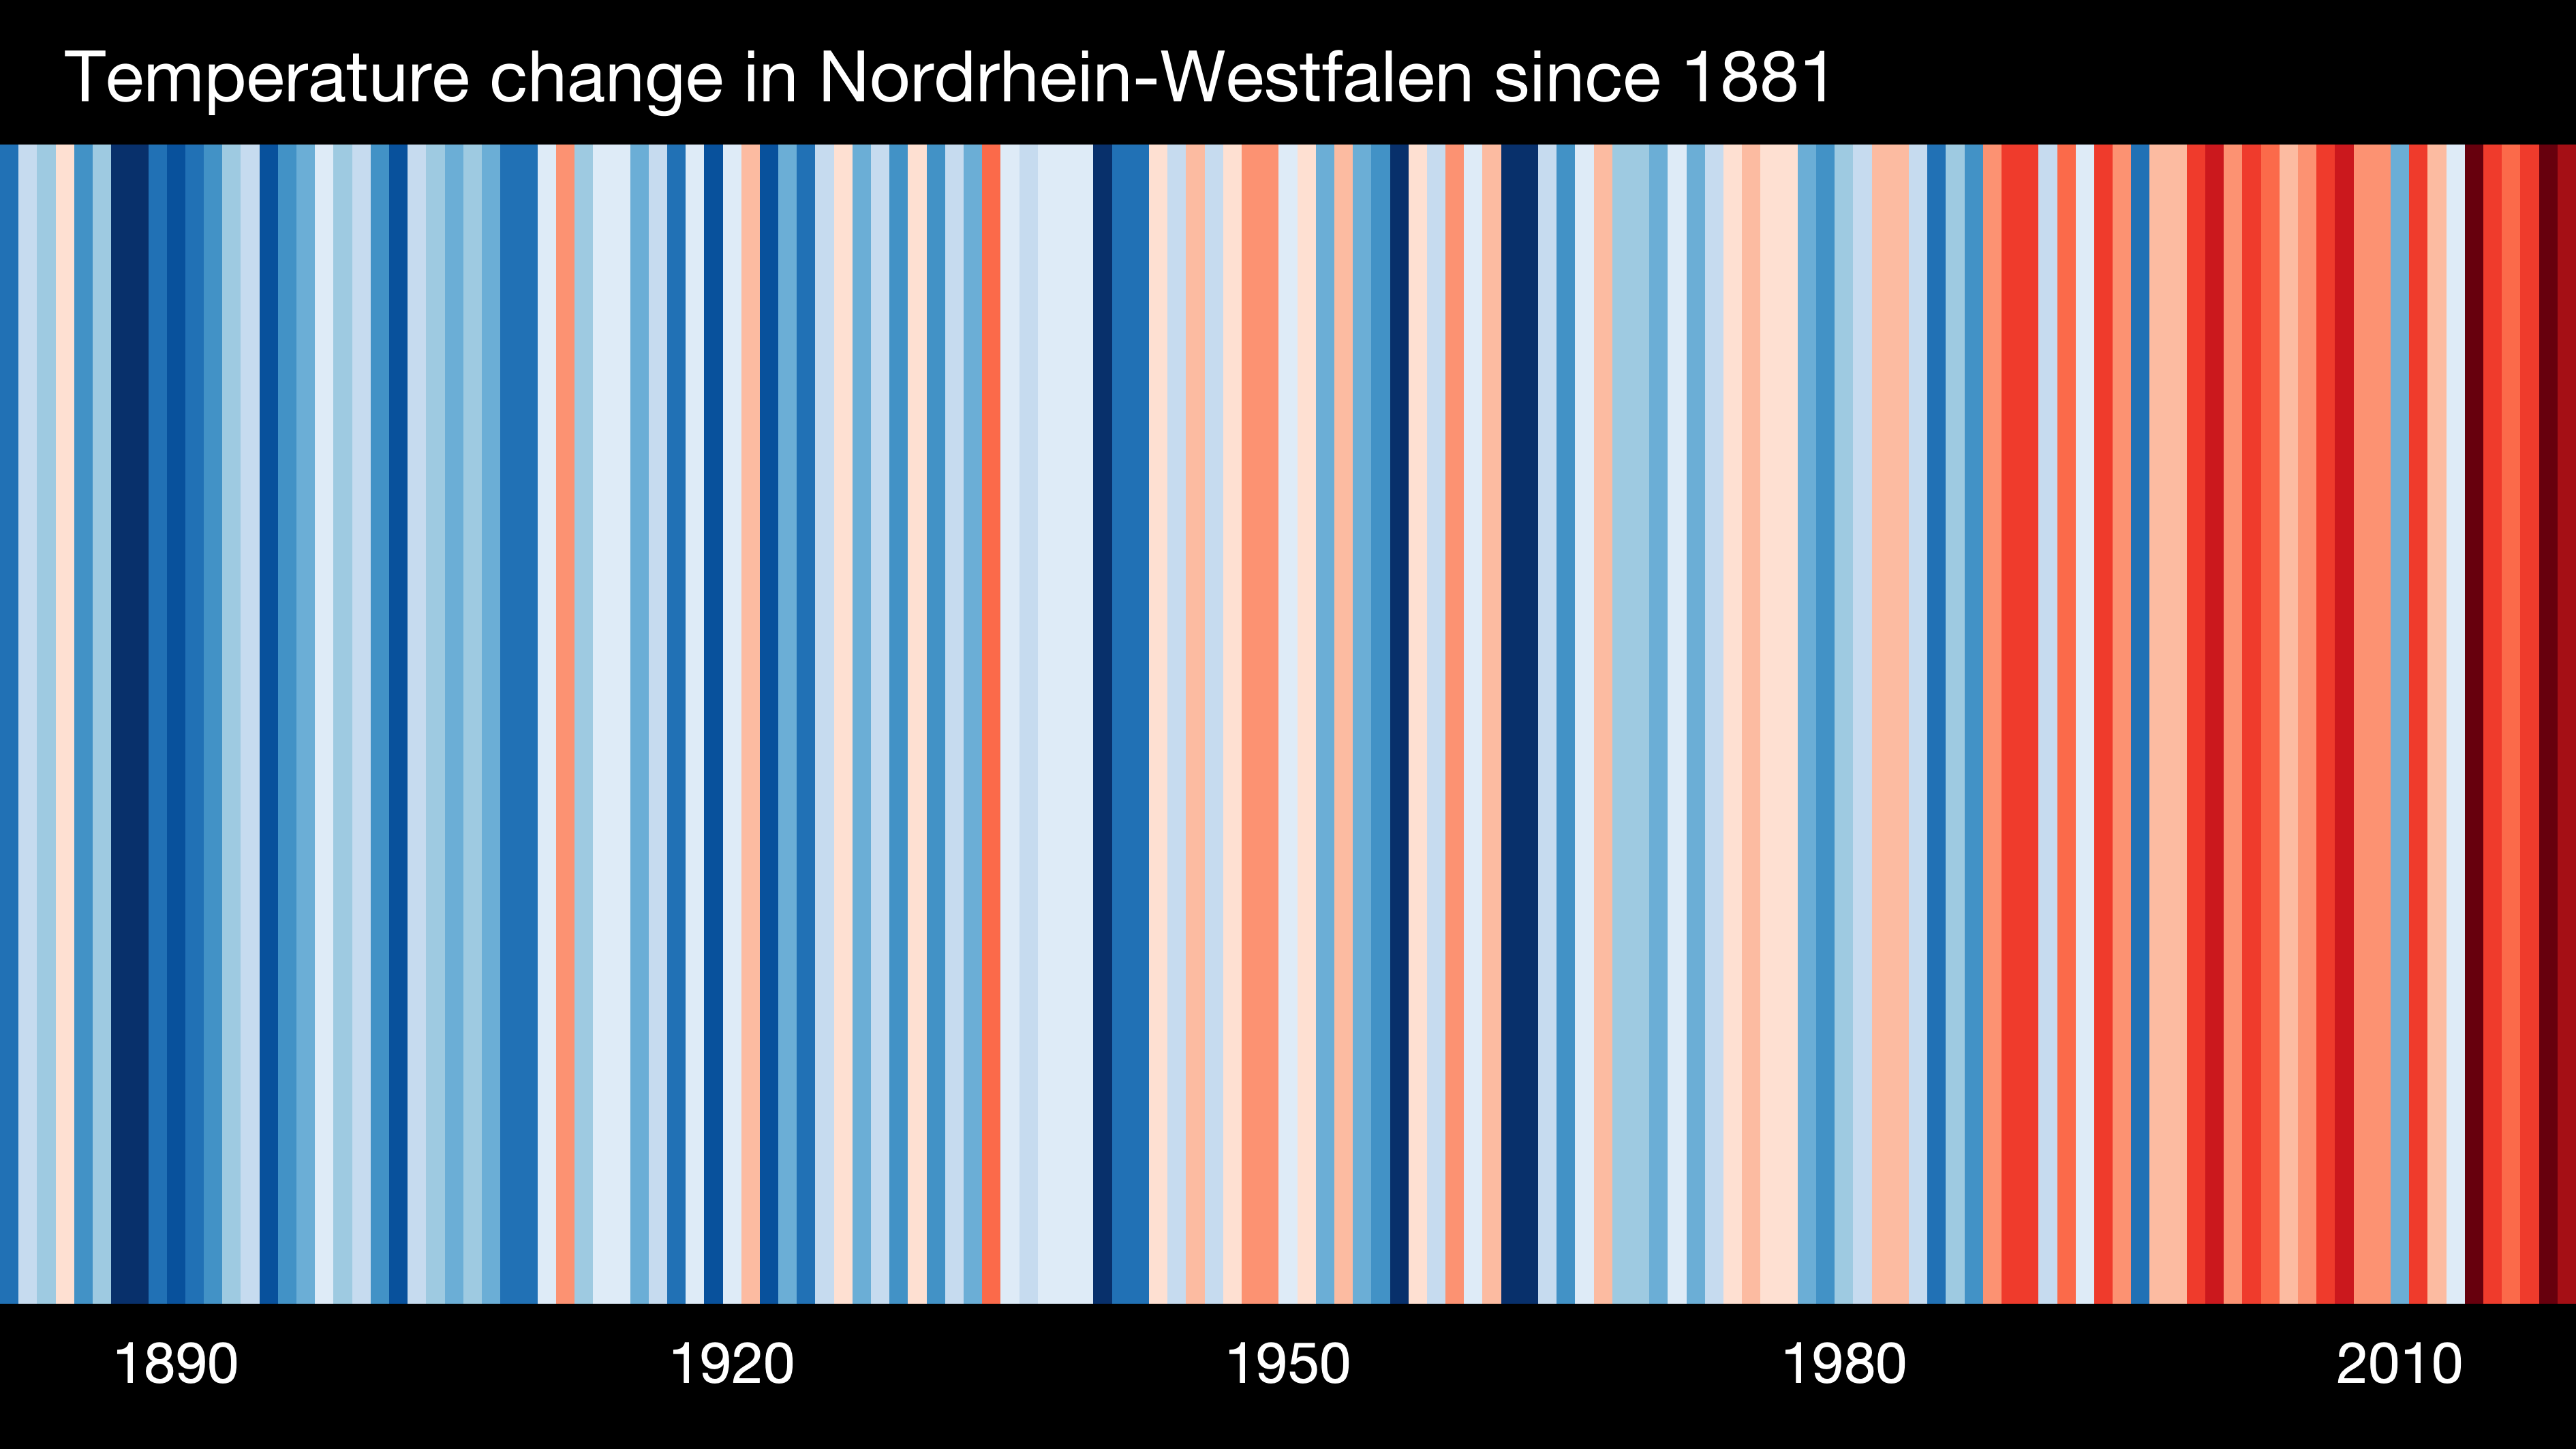
\includegraphics[width=\textwidth]{anhang/_stripes_EUROPE-Germany-Nordrhein_Westfalen-1881-2019-DW-withlabels.png}
	\caption[Titel der Figure]{Beschreibungstext Bla bla bla viel beschreiben sehr gut. \cite{Hawkins.2019}}
	\label{fig:DieLableIhAuhhNooo}
\end{figure}
